\documentclass[10pt]{extarticle} % Usa fonte de 10pt
\usepackage{graphicx} % Required for inserting images
\usepackage{float}
\usepackage{geometry}
\usepackage{hyperref}
\usepackage{minted}
\usepackage{bookmark}
\setminted{
  breaklines=true, % Permite quebra de linha
  breakanywhere=true, % Permite quebra em qualquer posição
  fontsize=\small % Define tamanho da fonte para ajudar com overflow
}

\geometry{margin=1in}

\title{Trabalho Prático 1 - Introdução a Inteligência Artificial}
\author{Francisco Teixeira Rocha Aragão - 2021031726}

\date{Data: 11 de Dezembro de 2024}

\begin{document}

\maketitle

\section{Introdução}

O presente trabalho busca exercitar os conceitos de busca em espaço de estados. Dessa forma, recebendo um mapa de cidades, suas respectivas coordenadas e custos em cada caminho, o objetivo é encontrar um caminho ligando o ponto inicial até o ponto final desejado. Assim, foram implementados diferentes algoritmos para resolução do problema, sendo BFS (Busca em Largura), UCS (Busca de Custo Uniforme), IDS (Busca em Profundidade Iterativa) além das heurísticas A* e uma abordagem gulosa. Com isso, abaixo encontram-se mais informações sobre a modelagem do problema, os algoritmos utilizados, detalhes de implementação além dos resultados e conclusões obtidas.

\section{Definição do problema}

O problema é constituído de uma matriz que representa os terrenos em cada posição do mapa, com o objetivo de encontrar um caminho entre o ponto inicial e final. Desse modo, o mapa foi representado como uma matriz de dimensões Linhas x Colunas, com cada posição contendo um valor que representa o terreno. Cada um dos algoritmos então realiza uma busca nessa matriz, levando em consideração os respectivos custos de cada tipo de terreno que foram fornecidos na descrição do trabalho. Assim, a classe 'Game' lida salvando as informações úteis sobre o mapa, junto de dados do percurso escolhido e os algoritmos de busca, o que é feito com o auxílio da classe 'Utils' que contém funções representando as heurísticas utilizadas e para receber informações do mapa.

\section{Algoritmos Implementados}

Vale destacar que para análise dos algoritmos abaixo, medidas de complexidade como 'b' (branch factor), 'd' (profundidade da solução mais rasa) e 'm' (profundidade máxima da busca) foram utilizadas em um contexto específico do problema, que não envolve árvores de busca, mas sim a matriz que representa o mapa do jogo. Desse modo, cada nó visitado expande nó máximo 4 vizinhos (cima, baixo, esquerda e direita) e a profundidade está restrita a área do mapa.

\subsection{Busca em Largura (BFS)}

O algoritmo de busca em largura é um algoritmo de busca sem informação que consiste em expandir todos os nós vizinhos do nó atual, ou seja, expande cada nível do mapa antes de passar para o próximo. Assim, o algoritmo verifica o nó inicial, depois expande os vizinhos de cima, baixo, esquerda e direita, e assim por diante. O algoritmo termina então ao ser encontrado o nó final. Esse algoritmo não é ótimo no trabalho atual, visto que o problema não possui uma função de custo crescente por nível (diferentes terrenos possuem custos diferentes). Dessa forma, o primeiro caminho que chega na solução já finaliza o algoritmo. Mesmo não sendo ótimo, o algoritmo é completo e encontra uma solução. Sua complexidade é de O(b\textsuperscript{d}) para tempo e espaço, em que b é o branch factor e d é a profundidade da solução mais rasa.

\subsection{Busca de Custo Uniforme (UCS)}

A busca de custo uniforme é um algoritmo de busca sem informação que expande o nó com menor custo total até o momento. É utilizado uma fila de prioridades (heap) para implementação, escolhendo e atualizando os nós descobertos a cada iteração, selecionando o melhor (de menor custo) para expansão. Justamente por essa escolha e atualização do melhor para expansão, o algoritmo é ótimo, e no caso do problema também é completo, já que não existem custos negativos nem ciclos. Sua complexidade depende do custo da solução ótima C*, sendo O(b\textsuperscript{1 + C*/e}), em que 'e' é o menor custo.

\subsection{Busca em Profundidade Iterativa (IDS)}

A busca de profundidade iterativa funciona executando uma DFS limitada por nível, explorando cada um dos níveis incrementalmente a cada iteração. Dessa forma, o algoritmo começa com uma profundidade 0, expandindo em profundidade todo o nível, depois reinicia o processo expandindo em profundidade o próximo nível. O algoritmo tem características semelhantes a BFS em respeito a otimilidade e competude (no caso do problema em questão, o algoritmo é completo mas não é ótimo). Sua complexidade de tempo é O(b\textsuperscript{d}) com espaço O(bd). O algoritmo realiza mais expansões de nós do que os demais, visto que revisita todos os nós anteiores a cada iteração, porém no limite esse custo é dominado pelo último nível expandido.

\subsection{Greedy}

A heurística de busca gulosa consiste em uma busca com informação, sendo utilizada uma heurística para auxiliar as tomadas de decisões. Assim, ao invés de se utilizar o custo real dos caminhos, é utilizado a distância heurística como métrica de escolha. Dessa forma, o caminho com menor valor para a função heurística é escolhido para ser expandido. O algoritmo não é ótimo (visto que não considera os custos reais) porém é completo (por padrão a abordagem não é completa, porém nesse trabalho sua implementação foi feita salvando caminhos já visitados, evitando que o algoritmo entre em loop). Sua complexidade é O(b\textsuperscript{m}), em que 'm' é a profundidade máxima da busca. No entanto, vale destacar que sua complexidade e performance também dependem da heurística utilizada.

\subsection{A*}

A abordagem A* novamente é um algoritmo de busca com informação que atua de modo semelhante a abordagem UCS, porém não considera somente os custos reais, mas também a função heurística para auxiliar a busca. Desse modo, o algoritmo expande o nó com menor custo total, sendo a soma do custo real e da função heurística. O algoritmo é completo (assim como UCS) e ótimo (desde que a heurística seja admissível, o que é o caso do problema em questão, em que será comentado na seção abaixo). Sua complexidade é semelhante a UCS, porém também é influenciada pela heurística utilizada.

\section{Heurísticas}

Abaixo estão detalhadas as duas heurísticas utilizadas no trabalho. Vale comentar que a heurística principal usada nos testes foi a distância euclidiana. Porém, mais ao fim na seção de resultados é apresentado um comparativo para o algoritmo guloso utilizando a distância euclidiana e a distância de manhattan.  

\subsection{Distância Euclidiana}

A função heurística utilizada primariamente no trabalho é a distância euclidiana entre dois pontos, sendo importante para guiar a busca dos algoritmos de busca com informação. A função é calculada a partir da fórmula: 

\begin{equation}
    h(n) = \sqrt{(x2 - x1)\textsuperscript{2} + (y2 - y1)\textsuperscript{2}}
\end{equation}

Essa função é uma heurística admissível, já que a distância euclidiana é sempre menor ou igual a distância real entre dois pontos. No problema em questão, isso também é válido visto que o importante não é somente a distância entre os pontos, mas também o custo de cada terreno que é percorrido. Dessa forma, o valor da heurística sempre vai ser menor que o custo real.

\subsection{Distância de Manhattan}

A distância de Manhattan é uma heurística admissível que calcula a distância entre dois pontos em um plano cartesiano, sendo a soma das diferenças absolutas entre as coordenadas x e y dos pontos. A fórmula é dada por:

\begin{equation}
    h(n) = |x2 - x1| + |y2 - y1|
\end{equation}

Assim como a distância euclidiana, a distância de Manhattan é uma heurística admissível, já que a distância no plano cartesiano equivale a distância real do mapa do problema (considerando que o terreno seja o de menor custo, ou seja, custo 1). Desse modo, a heurística é equivalente ao caminho real mais curto entre dois pontos, sendo que na prática por conta de caminhos mais caros, a heurística é sempre menor ou igual ao custo real.

\section{Execução e Resultados}

O código foi desenvolvido em Python versão 3.11.2 e os testes foram realizados em uma máquina com debian 12, 16GB de ram e processador I5-11 geração. Sua execução pode ser realizada com os seguintes comandos:

\begin{minted}{python}
// execução
python3 main.py <caminho para o arquivo de entrada> <algoritmo> <inicio_x> <inicio_y> <final_x> <final_y>

// medição de tempo e número de nós expandidos
python3 main.py <caminho para o arquivo de entrada> <algoritmo> <inicio_x> <inicio_y> <final_x> <final_y> --measure

// algoritmos -> BFS, IDS, UCS, AStar ou Greedy
\end{minted}

Vale destacar que como alguns dos algoritmos foram imlpementados de maneira recursiva, para instâncias maiores foi necessário aumentar o limite de recursão padrão do Python para permitir a execução dos testes.

Abaixo nas figuras 1 e 2 estão alguns resultados iniciais dos algoritmos em uma instância pequena. Como já esperado, o custo ótimo é encontrado pelo UCS, juntamente do A* que obteve um bom desempenho, com os demais algoritmos possuindo custos semelhantes, embora não ótimos. Sobre o tempo, como a instância é pequena, uma análise assim torna-se não muito útil, porém observando o número de nós expandidos, é possível perceber a tendência dos algoritmos com o Greedy sendo o mais direto até o destino final, acompanhado do A*, enquanto os demais precisam expandir mais nós.

\begin{figure}[H]
    \centering
    \begin{minipage}{0.5\linewidth}
        \centering
        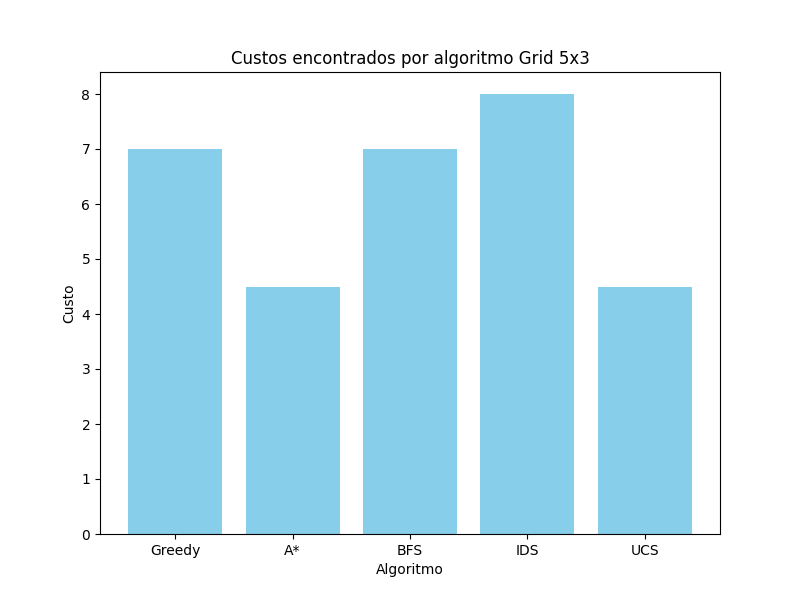
\includegraphics[width=\linewidth]{cost_per_algorithm_5x3.png}
        \caption{Custos para entrada 5x3}
        \label{fig:cost-per-algorithm}
    \end{minipage}%
    \begin{minipage}{0.5\linewidth}
        \centering
        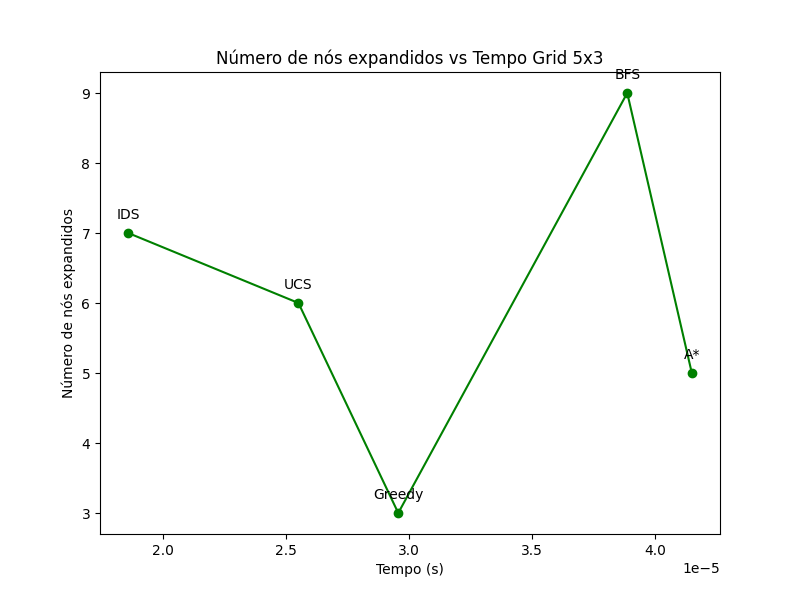
\includegraphics[width=\linewidth]{expanded_nodes_vs_time_labeled_5x3.png}
        \caption{Nós expandidos e tempo para entrada 5x3}
        \label{fig:expanded-nodes-vs-time}
    \end{minipage}
\end{figure}

De toda forma, mais testes foram executados para instâncias maiores conforme mostrado abaixo. Vale destacar um ponto importante, o algoritmo IDS obteve resultados muito ruins de performance, sendo praticamente inviável usá-lo na prática. Isso se deve ao fato de praticamente ser efetuado uma busca exaustiva em todo o espaço de busca (por conta do backtracking). Desse modo, sua execução foi ignorada.

Focando nos outros algoritmos presentes nas figuras 3 e 4, a fundamentação teórica foi comprovada agora em instâncias maiores com o ponto inicial sendo (1, 130) e o final (166, 192). O algoritmo Guloso mostrou-se o mais eficiente em questão de performance, obtendo o menor número de nós expandidos e também o menor tempo. No entanto, seus resultados não são tão bons. Em contraste, a BFS obteve resultados ruins, tanto no custo encontrado quanto em tempo e número de nós expandidos.

Vale destacar a comparação entre A* e UCS. Ambos obtiveram o resultado ótimo ao final da execução, no entanto, suas execuções ocorrem de maneira diferente. Por conta da heurística utilizada, o algoritmo A* possui uma execução muito mais precisa, expandindo menos nós e indo mais direto ao destino final em comparação ao UCS. Isso é válido ao se observar a figura 4 que mostra esse ganho de performance do A*.

\begin{figure}[H]
    \centering
    \begin{minipage}{0.5\linewidth}
        \centering
        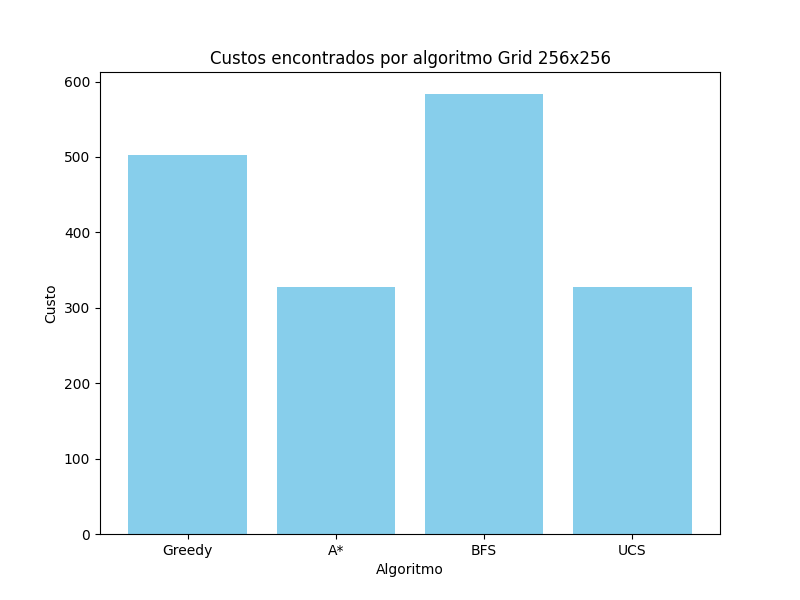
\includegraphics[width=\linewidth]{cost_per_algorithm_256x256.png}
        \caption{Custos - Instância Cidade 256x256}
        \label{fig:cost-per-algorithm}
    \end{minipage}%
    \begin{minipage}{0.5\linewidth}
        \centering
        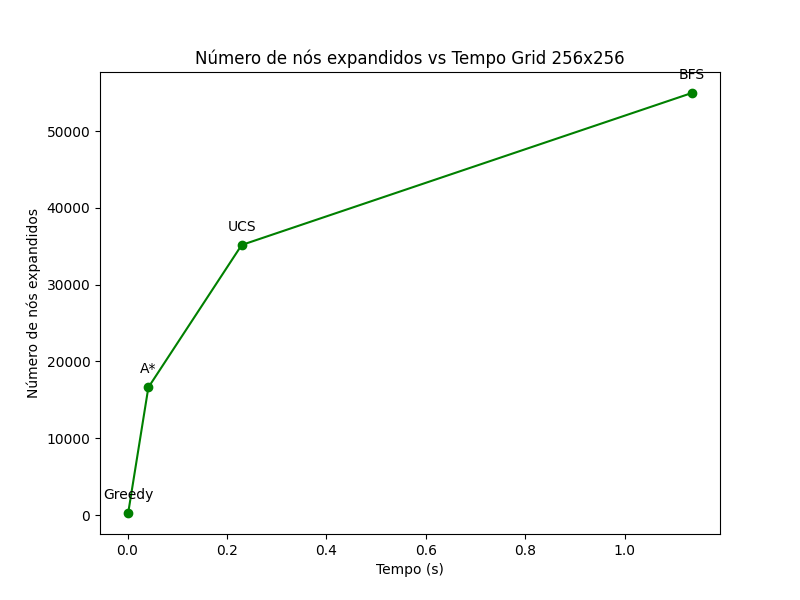
\includegraphics[width=\linewidth]{expanded_nodes_vs_time_labeled_256x256.png}
        \caption{Nós expandidos e tempo - Instância Cidade 256x256}
        \label{fig:expanded-nodes-vs-time}
    \end{minipage}
\end{figure}

No entanto, dado os bons resultados do algoritmo Guloso, vale ressaltar alguns dos problemas. Como exemplo, ele é um algoritmo totalmente baseado em heurísticas. Sendo assim, mesmo que a heurística aponte que determinado caminho seja promissor, na prática a situação pode ser completamente diferente. Com isso, percebe-se como o algortimo Guloso é pouco 'flexível' dado a instância recebida, sendo guiado cegamente pela heurística sem considerar as situações reais. Isso é visto nas figuras 5 e 6 presentes abaixo, executado a partir de (244, 21) até (104,2) em que mesmo com a boa performance em comparação aos demais, a algoritmo guloso obteve um custo final ruim.

\begin{figure}[H]
    \centering
    \begin{minipage}{0.5\linewidth}
        \centering
        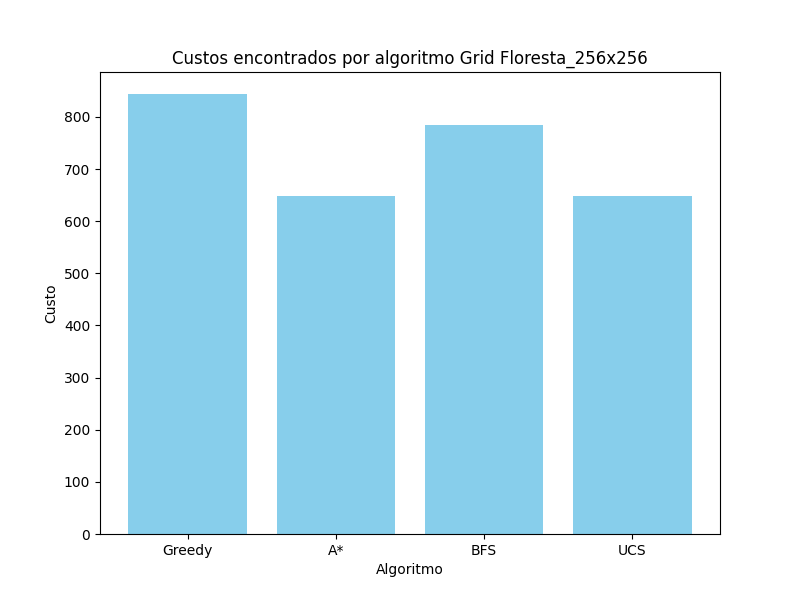
\includegraphics[width=\linewidth]{cost_per_algorithm_Floresta_256x256.png}
        \caption{Custos - Instância Floresta 256x256}
        \label{fig:cost-per-algorithm}
    \end{minipage}%
    \begin{minipage}{0.5\linewidth}
        \centering
        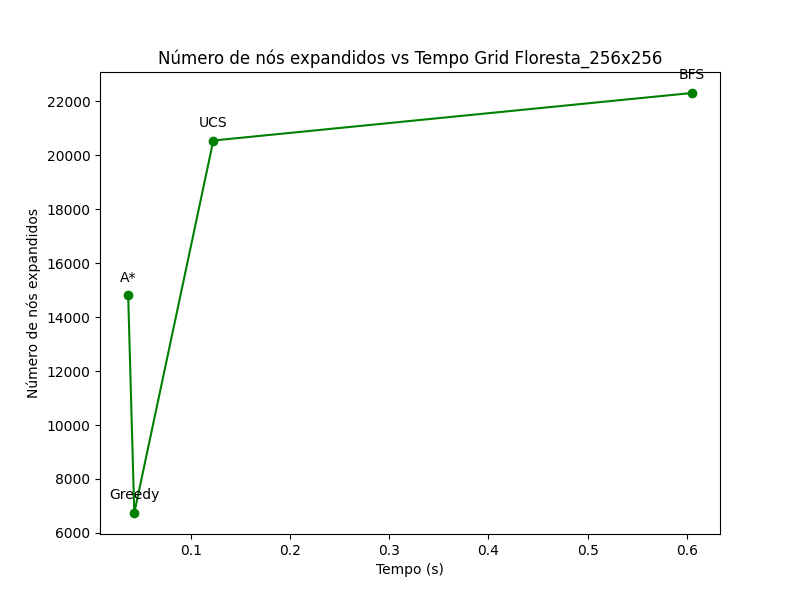
\includegraphics[width=\linewidth]{expanded_nodes_vs_time_labeled_Floresta_256x256.png}
        \caption{Nós expandidos e tempo - Instância Floresta 256x256}
        \label{fig:expanded-nodes-vs-time}
    \end{minipage}
\end{figure}

Novamente sobre o algoritmo guloso, vale destacar como o uso da heurística influencia no seu desempenho. Dessa forma, o algoritmo ao seguir cegamente a heurística, acaba indo para caminhos potencialmente ruins, ou que estão bloquados por exemplo. Assim, o comportamento esperado seria de que a cada iteração, o próximo ponto escolhido seja mais próximo do destino final. No entanto, como mostrado na figura 7 abaixo, isso não é a realidade, com o algoritmo em alguns momentos escolhendo os próximos vizinhos que não estão se aproximando do nó final em comparação ao nó atual, justificado assim por conta do algoritmo escolher distâncias ruins anteriormente que levam a caminhos não promissores. 

\begin{figure}[H]
    \centering
    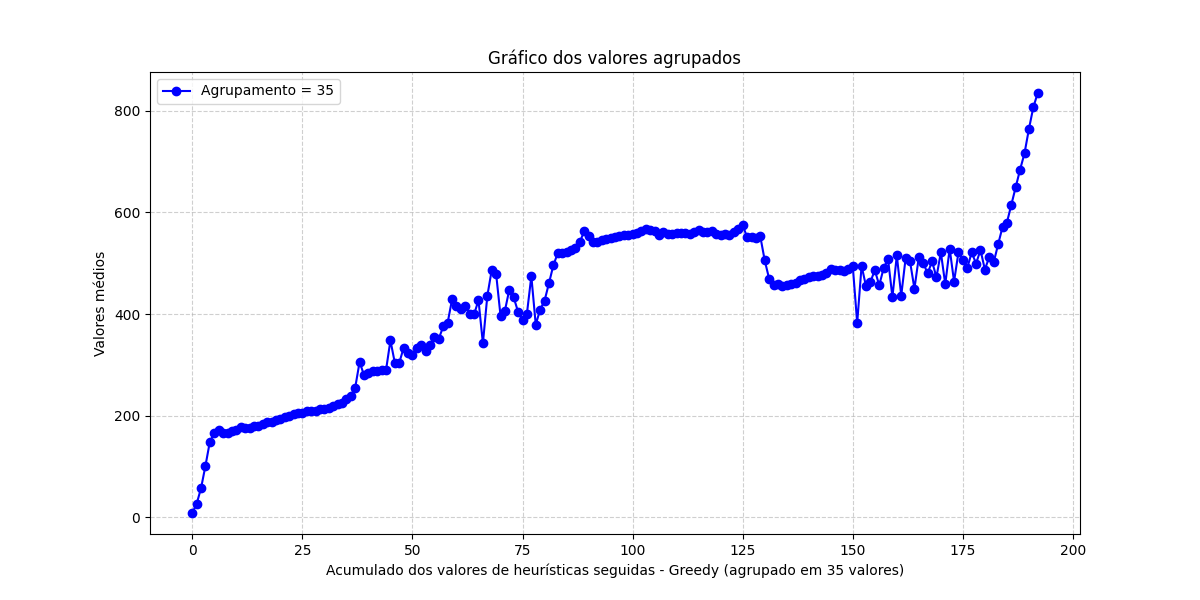
\includegraphics[width=0.9\linewidth]{greedy_alg_dist_cumulative.png}
    \caption{Distâncias euclidianas escolhidas em cada iteração - Greedy}
    \label{fig:enter-label}
\end{figure}

Desse modo, ao trocar a função heurística da distância euclidiana pela distância de manhattan, percebe-se na imagem 8 como os caminhos escolhidos tornam-se mais 'comportados', indo de encontro ao nó objetivo a cada iteração. Isso é válido pois a distância de manhattan obtêm valores maiores em comparação a distância euclidiana, sendo uma heurística melhor para ser usada. Verifica-se então essa influência na tabela 1 apresentada abaixo, com as diferenças dos resultados para cada heurística na abordagem gulosa, mostrando como o desempenho é melhor como já previsto.

\begin{figure}[H]
    \centering
    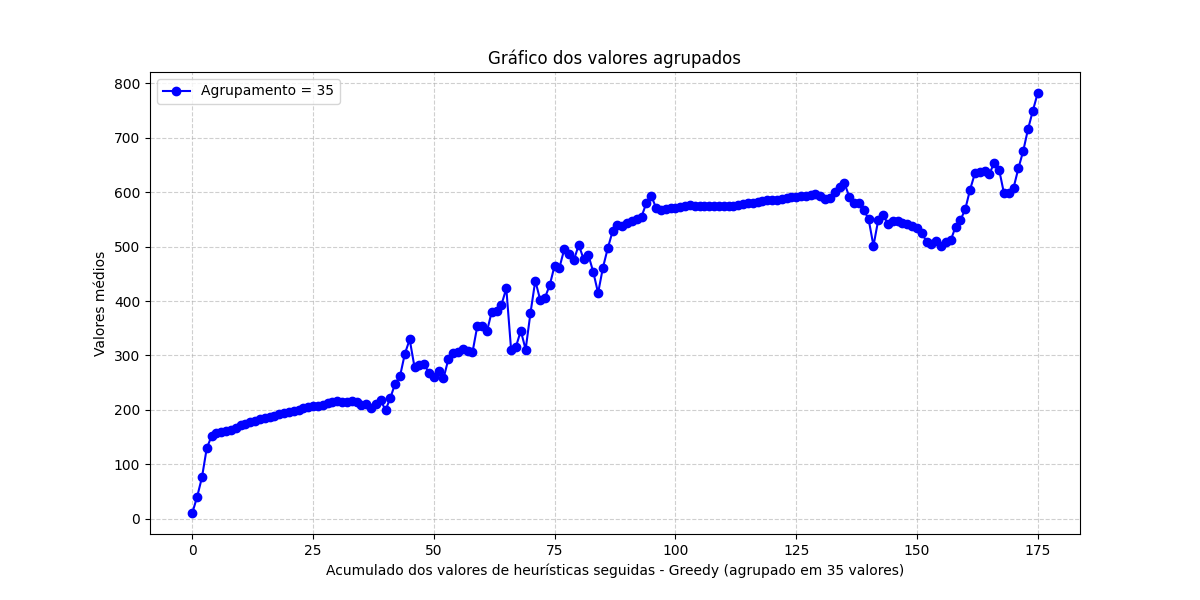
\includegraphics[width=0.9\linewidth]{greedy_alg_dist_cumulative2.png}
    \caption{Distâncias de manhattan escolhidas em cada iteração - Greedy}
    \label{fig:enter-label}
\end{figure}

\begin{table}[h]
    \centering
    \begin{tabular}{|c|c|c|c|} \hline 
         \textbf{Heurística} & \textbf{Nós expandidos} & \textbf{Tempo} & \textbf{Custo encontrado}\\ \hline 
         Manhattan      & 6155    & 0.03737     & 797.0    \\ \hline
         Euclidiana  & 6739    & 0.04278     & 844.0   \\ \hline
    \end{tabular}
    \caption{Comparação algoritmo Guloso com distância de Manhattan e Euclidiana}
    \label{tab:comparison_with_initial}
\end{table}


\section{Conclusão}

Ao final dos experimentos, foi possível observar a utilidade do trabalho para reforçar conceitos de funcionamento de cada algoritmo. Percebe-se na prática que busca em espaço de estados é um problema complicado, que facilmente consegue obter um número exponencial de possibilidades. Desse modo, a utilização de heurísticas são de grande auxílio para melhorar a performance, embora devam ser usadas com cuidado. Nesse caso, o algoritmo A* mostrou-se muito eficiente, comparativamente ao UCS que apresentou bom desempenho e resultados ótimos, o A* conseguiu fazer o mesmo com uma performance melhor, mostrando como heurísticas aliadas ao custo real auxiliam na tarefa. 

Vale destacar também que buscas exaustivas não são boas opções em grandes espaços de estado, como é o caso da BFS e principalmente IDS que tiveram resultados ruins de performance e no caso da IDS nem foi possível realizar sua execução. Tal fato motiva futuros trabalhos, explorando métodos mais eficientes para completar a tarefa ou então utilizando implementações que viabilizem o uso de tais abordagens exaustivas.

\section{Referências}

\noindent \href{https://www.geeksforgeeks.org/depth-first-search-or-dfs-for-a-graph/}{Depth First Search Python - GeekforGeeks}

\noindent \href{https://www.datacamp.com/tutorial/depth-first-search-in-python}{Depth First Search Python - DataCamp}

\noindent \href{https://academy.finxter.com/python-iterative-deepening-depth-first-search-dfs-algorithm/}{Iterative Deepening Depth First Search Python - Finxter}

\noindent \href{https://www.geeksforgeeks.org/iterative-deepening-searchids-iterative-deepening-depth-first-searchiddfs/}{Iterative Deepening Depth First Search (IDDFS) - GeeksforGeeks}

\noindent \href{https://www.datacamp.com/tutorial/dijkstra-algorithm-in-python}{Dijkstra Algorithm in Python - DataCamp}

\noindent \href{https://www.geeksforgeeks.org/breadth-first-search-or-bfs-for-a-graph/}{Breadth First Search (BFS) for a Graph - GeeksforGeeks}

\noindent \href{https://www.geeksforgeeks.org/print-the-dfs-traversal-step-wise-backtracking-also/}{DFS Traversal Step-Wise with Backtracking - GeeksforGeeks}


\end{document}